\begin{center}
  \begin{tabular}{rl}
  % after \\: \hline or \cline{col1-col2} \cline{col3-col4} ...
  论文地址:& \href{https://arxiv.org/abs/1511.05493}{https://arxiv.org/abs/1511.05493} \\
  源码地址:& \href{https://github.com/yujiali/ggnn}{ggnn} (coded in Lua) \\
  slides:& \href{http://www.cs.toronto.edu/~yujiali/files/talks/iclr16_ggnn_talk.pdf}{ggnn-talk}\\
  关键词:& \textbf{RNN, Graph Sequential tasks} \\
  写于:& \date{2020-09-28}
  \end{tabular}
\end{center}

这篇论文\cite{li2015gated}提出了一种基于GRU\cite{cho2014learning}的GNN,能够进行输出单个值的任务(如结点分类、图分类等),也能完成\textbf{序列输出}的任务(如最短路、欧拉环等)。论文中使用bAbI\cite{weston2015aicomplete}(bAbI是Facebook AI推出的文本理解/推理任务生成器)任务和程序验证的任务对GG-NN, GGS-NN进行了测试均达到了很好的效果。
\par 论文中讨论的是针对有向图的GNN。那么是如何表示有向图的GNN呢?\\
对于有向图$\mathcal{G} = (\mathcal{V}, \mathcal{E})$,其邻接矩阵由两部分组成$A=[A_{in}, A_{out}]$,$A_{in},A_{out}$分别为入,出邻接矩阵。$\mathcal{G}$中每个结点$v$都定义了其$IN$和$OUT$结点集,分别表示指向$v$的边的起始结点集和从$v$出发的边的终点结点集。$v$的邻居结点集$NBR$定义为$IN \cup OUT$,并且对于边和结点都可以有各自的标签。
\par 论文中对GNN进行了回顾。GNN将图数据映射到输出的过程中,可以划分为两个部分:PROPAGATION MODEL, OUTPUT MODEL,分别用来计算节点的表征和将节点表征映射到输出。
\par 论文针对非序列的输出和序列的输出分别提出了GG-NNs(Gated Graph Neural Networks)和GGS-NNs(Gated Graph Sequence Neural Networks)。其中GG-NNs是基于GNN的,不同的是使用了GRU来构建PROPAGATION MODEL 和 OUTPUT MODEL。用于输出序列的GGS-NN则是在GG-NN的基础上构建的。接下来先介绍一下GRU\cite{cho2014learning},在介绍GG-NN和GGS-NN。
\paragraph{GRU(Gated Recurrent Unit)} 门控循环单元。GRU可以视为LSTM的变体,与LSTM很相似。与常规的RNN中的单元相比,门控神经单元间的连接是不变的,但每个门控神经单元内部都是经过精心设计的。作为门控RNN能够学会决定何时清除状态。
\begin{figure}[h]
    \centering
    \subfigure[LSTM cell]{
        \label{fig:lstm_cell}
        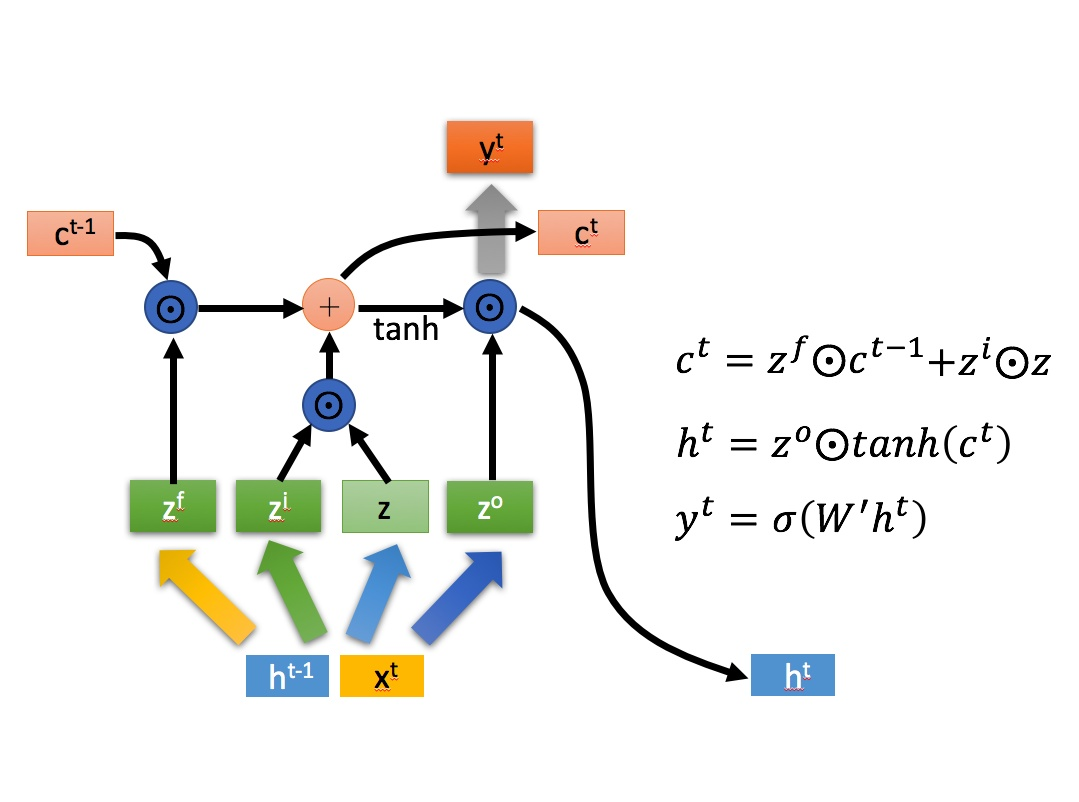
\includegraphics[width=.57\textwidth]{pics/LSTM.jpg}}
    \hspace{1.5pt}
    \subfigure[GRU cell]{
        \label{fig:gru_cell}
        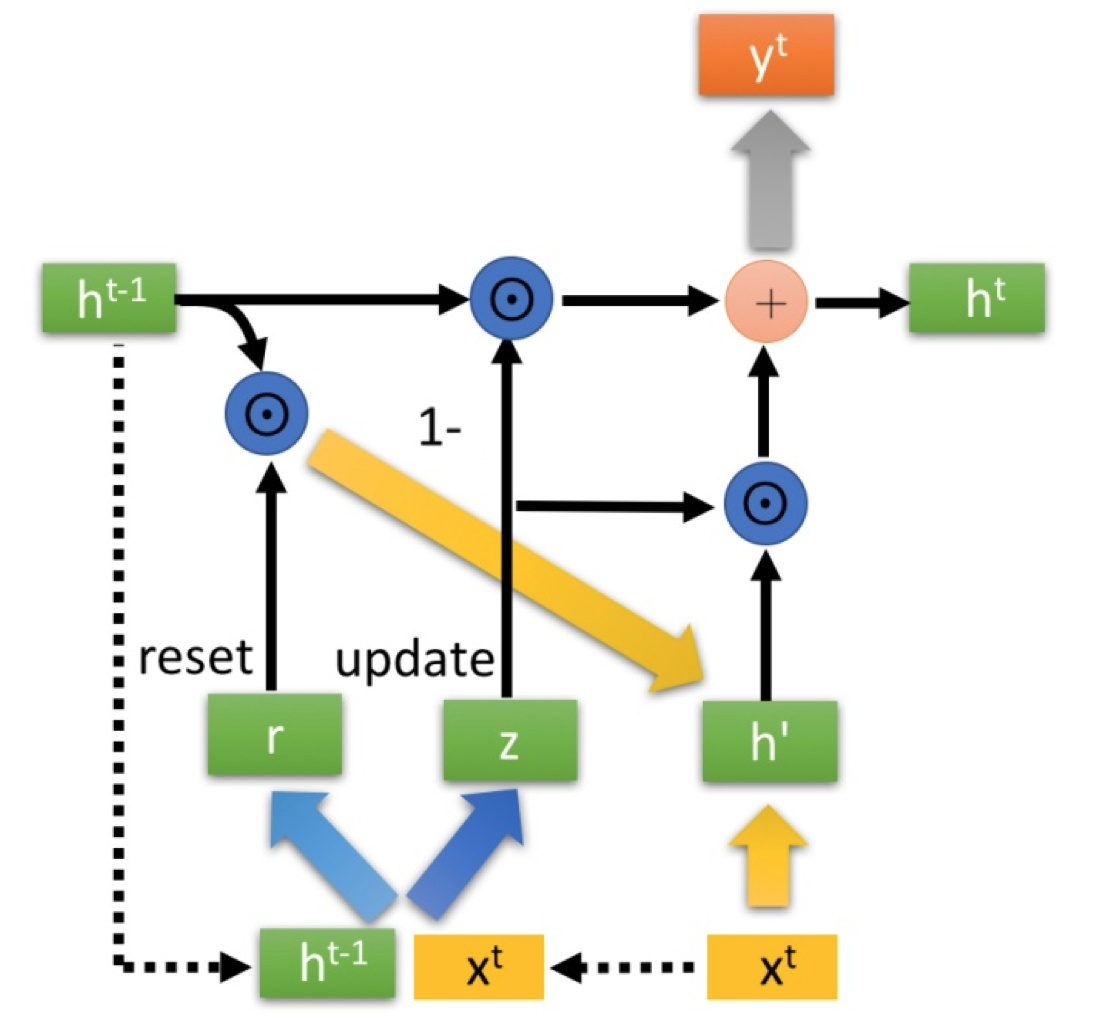
\includegraphics[width=.4\textwidth]{pics/GRU.jpg}}
    \caption{LSTM 和 GRU cell的内部结构}
    \label{fig:cell}
\end{figure}

\paragraph{GG-NN} GG-NN 的过程如下图所示。
\begin{figure}[h]
    \centering
    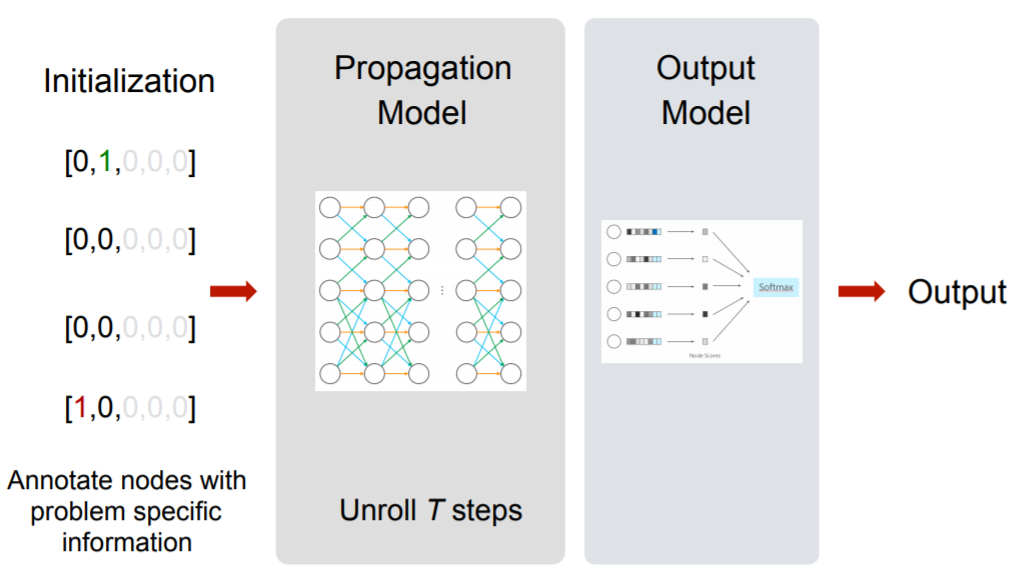
\includegraphics[width=.66\textwidth]{pics/ggnn.png}
    \caption{GG-NN}
    \label{fig:gg-nn}
\end{figure}
从Fig.\ref{fig:gg-nn}中可以看出,GG-NN的输入是 "Annotate nodes with problem specific information",在论文中称为"Node Annotations",这与之前提到的结点标签并不是同一个,node annotations 是在特定问题下所定义的“标签/特征”。根据特定的问题领域会为每个节点生成annotation({\color{red}如何生成annotations?}),在输入层会将annotation用0填充成固定的大小作为网络的输入。结点的annotations通过PROPAGATION MODEL---基于GRU的t层({\color{red}论文中成t-steps, 但根据我的理解是指网络有t层})网络,再将计算后的数据通过OUTPUT MODEL输出任务结果。

\paragraph{GGS-NN} GGS-NN 的过程如下。
\begin{figure}[h]
    \centering
    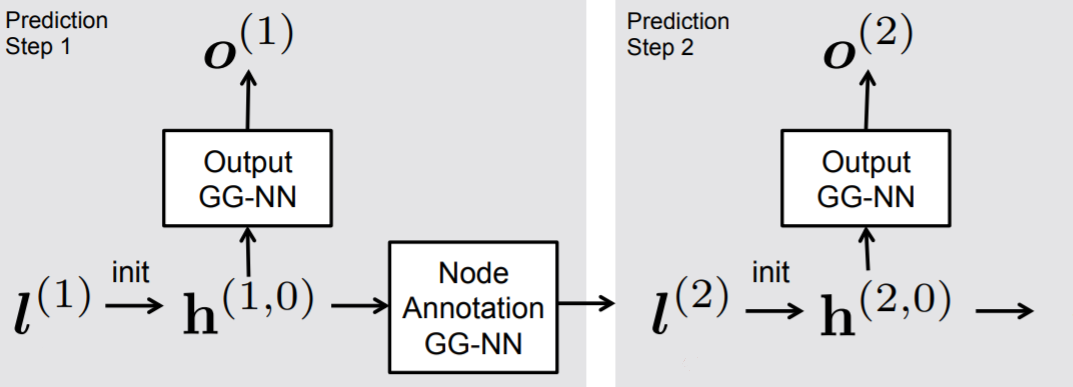
\includegraphics[width=.6\textwidth]{pics/GGS-NN.png}
    \caption{GGS-NN}
    \label{fig:ggs-nn}
\end{figure}
从Fig.\ref{fig:ggs-nn}中也能看出,GGS-NN是在GG-NN的基础上搭建的。GGS-NN的输入也是Node Annotations。每一步输入的Annotations是根据上一步的的隐层的输出转换而来的。每一步中的隐层输出会分别传给两个GG-NN,一个用来产生这一步的输出,另一个则用来产生下一步的输入,即下一步输入的node annotations。其实,在GGS-NN中除了上述两个GG-NN外,还有一个GG-NN用于在每一步确定是否继续,该GG-NN会在graph-level(把图看成一个特殊的结点,与图中的所有结点都有联系)上来进行一个二分类。

\par 论文中使用bAbI任务和程序逻辑验证进行测试。bAbI任务中将实体和实体间关系看作点和边(有点类似知识图谱),利用GG-NN/GGS-NN来进行推理。为解决程序验证中的program invariants 问题是这篇论文的一个主要出发点。通过将程序运行过程中heap的状态看作图数据,在这些数据的基础上以序列的方式生成程序的sepration logic\cite{10.1007/3-540-44802-0_1} 表达式。
\newline
网络参考资料:
\begin{enumerate}
    \item \href{https://www.jiqizhixin.com/articles/2017-12-24}{门控循环单元(GRU)的基本概念与原理}
    \item \href{https://towardsdatascience.com/illustrated-guide-to-lstms-and-gru-s-a-step-by-step-explanation-44e9eb85bf21}{Illustrated Guide to LSTM’s and GRU’s: A step by step explanation}
\end{enumerate}




